\documentclass[a4paper,ngerman]{tui-algo-seminar}
\usepackage{graphicx}
\usepackage{algorithm2e}
\usepackage{booktabs}
\usepackage{tikz}
\usepackage{hyperref}
\usepackage{float}
\usepackage{amsmath}
\usepackage{xskak}
\usepackage{listings}
%%\usepackage[margin=1in]{geometry}
\setlength{\footskip}{13.0pt}
\usepackage{thm-restate}
\lstset{
  basicstyle=\ttfamily,
  columns=flexible,
  breaklines=true 
}
\usepackage[utf8]{inputenc}

\newcommand{\inhalt}{Thüringer Jugend Einzelmeisterschaft 2024}
\seminar{\inhalt}
\semester{\today}
\title{\inhalt}
\author{Erik Skopp}

\usepackage{fancyhdr}
\pagestyle{fancy}
\fancyhf{}
\nolinenumbers

\begin{document}

\maketitle
\thispagestyle{plain}
\begin{abstract}
    Bericht: \inhalt.\\
    Vom 4. bis zum 7. April fand in Naumburg (Sachsen-Anhalt) die diesjährige Thüringer Jugend-Einzelmeisterschaft im Schach statt. In jeder Altersklasse wurden sieben Runden nach dem Schweizer System ausgetragen. Die Gewinner qualifizieren sich für die Deutsche Einzelmeisterschaft in Willingen.
\end{abstract}

%\listoffigures
%\listoftables
\tableofcontents 

\clearpage

\section{Bericht}

Vom vierten bis zum siebten April fand in Naumburg die diesjährige Thüringer Jugendeinzelmeisterschaft im Schach statt. In den Altersklassen U10 bis U18, sowohl männlich als auch weiblich, maßen sich die Kinder und Jugendlichen, um nicht nur gute Ergebnisse zu erzielen, sondern auch die Chance zu nutzen, sich für die deutsche Meisterschaft zu qualifizieren. Die jüngsten Teilnehmer in der Altersklasse U10 männlich absolvierten neun Runden, während alle anderen Kategorien sieben Runden spielten. Das gesamte Turnier wurde von der Thüringer Schachjugend organisiert.

In jeder Altersklasse hatte der Sieger die Möglichkeit, sich direkt für die Teilnahme an der deutschen Meisterschaft in Willingen zu qualifizieren. Falls im Vorjahr bereits Teilnehmer der jeweiligen Altersklasse auf dem Podium standen, hatten im darauffolgenden Jahr ein bis zwei weitere Spieler aus derselben Kategorie die Gelegenheit, an der deutschen Meisterschaft teilzunehmen. Die Thüringer Meisterschaften sind daher immer ein bedeutendes Ereignis. Für die Turnierteilnehmer wurden Vollverpflegung und Unterbringung in Gruppenzimmern bereitgestellt. Da das Frühstück bereits um sieben Uhr morgens serviert wurde und das Abendessen erst um halb sieben Uhr stattfand, waren die Tage sehr lang, was die Ausdauer der Kinder beeinträchtigte.

Kashvi Ray vertrat uns in der U10 weiblich. Mit einer Turnierwertungszahl (TWZ) von 758 ging sie als eine der Spielerinnen mit der drittniedrigsten Bewertung in ihrer Altersklasse ins Rennen, die aus 12 Teilnehmern bestand. Ursprünglich vom vierten Startplatz aus startend, beendete sie das Turnier leider auf dem neunten Platz. Sie startete das Turnier erfolgreich mit einem Weißsieg über Cäcilia Ulbrich in der ersten Runde. Dieser Sieg unterstreicht ihr Potenzial, das sich mit weiterem Training noch stärker entfalten könnte. In den Runden zwei und drei hatte Kashvi weniger Glück und verlor gegen Amalia und Amelia, die beide höhere Wertungszahlen hatten. In der vierten Runde gelang ihr jedoch ein Sieg gegen Elenor von Blau Weiß Stadtilm, der das Blatt wendete. Eine unglückliche Niederlage erlitt sie in der fünften Runde gegen Julia aus Saalfeld. In den letzten beiden Runden mobilisierte sie ihre Kräfte erneut und erreichte jeweils ein Remis gegen Fenja Nöthlich und Emily Fischer. Mit insgesamt 3 Punkten aus 7 Spielen landete sie auf einem durchwachsenen neunten Platz. Ihre DWZ konnte sie leider nicht bestätigen und verlor 20 Punkte, was sie von 758 auf 738 fallen ließ. Obwohl eine Qualifikation für die Deutsche Meisterschaft nicht erreicht wurde, sammelte Ronika wertvolle Erfahrungen, die ihr helfen sollen, im kommenden Jahr in ihrer Altersklasse zu dominieren.

In der U12w spielte Ronika Nasiri für uns. Es war ihr zweiter Anlauf bei der Thüringer Einzelmeisterschaft. Trotz ihres Engagements und ihrer Leidenschaft für das Spiel startete Ronika leider immer noch ohne eine Wertungszahl und fand sich daher auf dem 14. Platz wieder. Der Beginn des Turniers erwies sich für Ronika als äußerst herausfordernd, da sie mit zwei aufeinanderfolgenden Niederlagen in die erste Runde startete. Dies bedeutete einen holprigen Beginn, der ihre Moral auf eine harte Probe stellte. Doch in Runde drei ergriff sie die Gelegenheit und zeigte gegen Daria Kührt von Empor Erfurt, dass sie durchaus kämpfen konnte, indem sie ihren ersten Punkt gewann. Dieser Erfolg brachte jedoch nur vorübergehende Erleichterung, da das Glück in den nächsten Runden nicht auf ihrer Seite war. In Runde vier erlebte Ronika eine unglückliche Niederlage gegen Paulina aus Oldisleben, was ihre Motivation zusätzlich beeinträchtigte. Die nächste Begegnung gegen Clara Teres von Empor markierte ihr drittes Aufeinandertreffen mit einem Spieler von Empor. Bedauerlicherweise unterlag sie

 erneut, und zwar recht schnell, was zu einem weiteren Rückschlag führte. Trotz dieser Herausforderungen ließ sich Ronika nicht entmutigen und kämpfte weiter. In Runde sechs zeigte sie eine bemerkenswerte Leistung und sicherte sich einen deutlichen Sieg gegen Ellen, was ihre Entschlossenheit und ihren Kampfgeist unter Beweis stellte. Die letzten beiden Runden des Turniers waren geprägt von Erschöpfung und Anstrengung, da Ronika die physischen und mentalen Belastungen spürte, die mit einem Schachturnier einhergehen. In diesen letzten beiden Runden trat sie gegen Clara an und verlor, womit sie gegen die vierte Teilnehmerin aus Erfurt unterlag. Mit zwei Punkten aus sieben Runden konnte Ronika die Erwartungen nicht erfüllen, doch immerhin gelang es ihr, ihren Startplatz von Platz 14 auf Platz 12 zu verbessern. Durch ihre Teilnahme an der Thüringer Einzelmeisterschaft der Jugend erhielt sie ihre erste DWZ, die mit 763 bewertet wurde. Diese Zahl stellt einen Anfang dar und bietet viel Potenzial für weitere Verbesserungen, insbesondere durch kontinuierliches Training und Engagement. Wir möchten Ronika für ihren Einsatz und ihre Hingabe während des Turniers loben und ihr für das kommende Jahr viel Erfolg und Fortschritt wünschen.

Hanna Görlach tritt dieses Jahr zum ersten und letzten Mal für Ilmenau in der Altersklasse U18 weiblich an. Die Mädchen der Altersklasse U14 bis U18 spielten zusammen in einer eigenen Gruppe, diese wurde am Ende jedoch getrennt gewertet. Hanna startete in der herausforderndsten Altersklasse vom 9. Platz aus, mit einer TWZ von 1122. Das Turnier begann vielversprechend für sie, mit einem Pflichtsieg in Runde 1 gegen Anna Grube aus Meiningen. In der zweiten Runde lieferte sie sich einen langen Kampf, den Hanna dominierte, und erreichte ein Remis gegen Celine Brauer vom SC Turm Erfurt. Dieses Remis sollte sich bald wiederholen. Trotz einer Wertungszahl von 1464 gelang es Hanna, ein wichtiges Remis mit den schwarzen Steinen gegen Gabriela Ignatova aus Meuselwitz zu erreichen, nach einem guten Start mit 1,5 Punkten aus 2 Runden. Das Glück verließ Hanna jedoch gegen Stadtilm, wo sie unglücklich gegen Amelie Elsa verlor. In den Runden fünf und sechs folgten schmerzhafte Niederlagen mit jeweils 2 Remis gegen Fabienne Huth aus Gera und Selma Zeughardt vom Erfurter Schachklub, beide mit einer DWZ von jeweils 1000. Leider konnte sich Hanna davon nicht erholen und verlor in der letzten Runde gegen Sophia Scheiding aus Meuselwitz. Diese Ergebnisse führten leider zu einem DWZ-Minus von 30 Punkten und einer Verschlechterung ihres Startplatzes auf Rang 13. Da in der Altersklasse U18 weiblich nur 2 Teilnehmer sind, Helena Ulrich und sie qualifizierte sich Helena für die Deutsche Meisterschaft. Da diese jedoch nicht möchte, rückt Hanna nach und darf zur Deutschen Einzelmeisterschaft nach Willingen fahren. Diese Leistung in diesem Turnier war jedoch nur ein Ausrutscher. Nach ihren großen Erfolgen beim Grenke Open hatte Hanna noch keine Ruhepause. Diese fehlende Ruhe spiegelte sich in ihrer Ausdauer und Konzentration wider. Hier zeigt sich deutlich, dass Schach auch ein Sport ist. Ich bin zuversichtlich, dass sie sich nach dem Turnier durch hartes Training wieder nach oben kämpfen und erneut Erfolge erzielen kann.

Keines der Kinder konnte die Erwartungen erfüllen. Trotz intensivem Training konnte keines der Kinder durch eigene Leistung eine Qualifikation zu der Deutschen Meisterschaft erringen. Dies ist nicht schlimm, denn so wurde uns gezeigt, welche Baustellen die Kinder noch haben und wo man im Training ansetzen kann. Insbesondere hat sich hier die Ausdauer und Zeitverwaltung der Kinder gezeigt. Insbesondere die jüngeren hatten durch das Inkrement von 30 Minuten mitunter mehr Zeit auf der Uhr als am Anfang. Dass dies nicht zu besten Zügen und erfolgreichen Partien füh

rt, zeigt sich schnell. Auch wenn die Ergebnisse hinter den Erwartungen zurücklagen, war es ein guter Test für die Kinder, ihre eigenen Fähigkeiten im Rahmen eines Turniers unter Beweis zu stellen. Mit ausreichend Training und dem Willen, etwas zu lernen, erreichen die Kinder im kommenden Jahr ihre Ziele.

Das Turnier begann mit dem üblichen Trubel bei Turnieren mit Kindern. Im Großen und Ganzen hat das Turnier den Kindern Spaß gemacht und sie an die Welt des praktischen Schaches herangeführt. Wir trauen unseren Spielern zu, sich im Laufe des kommenden Jahres zu verbessern und die Ergebnisse aus diesem Jahr zu überflügeln.


\vspace{2cm}
Erik Skopp\\
Ilmenauer Schachverein\\
\clearpage


\section{Tabellen}
Alle Tabellen entstammen der Veröffentlichung der Thüringer Schachjugend unter folgender URL \url{https://ed.thsj.de/index.php/them-2024}\footnote{Der Link wurde am \today ~abgerufen.}

% Auch wenn die Pfade nicht stimmen findet Overleaf die Projekte. Bei GitHub und dem Worfkflow ist das nicht so,
\subsection{Hanna Görlach}
    \subsubsection{Partien}
        \begin{table}[htbp]
\centering
\caption{Turnier Rangliste}
\begin{tabular}{|l|c|l|l|c|c|}
\hline
\multicolumn{6}{|c|}{Partien} \\
\hline
Runde & Farbe & Spieler & Verein & ELO & Ergebnis \\
\hline
1 & W & Grube, Anna (2.5) & ESV Lok Meiningen & 841 & 1 \\
2 & S & Brauer, Celiene (4) & SC Turm Erfurt & 1172 & 0.5 \\
3 & S & Ignatova, Gabriela (4.5) & Meuselwitzer SV & 1464 & 0.5 \\
4 & W & Richter, Amélie Elsa (4) & SG Blau-Weiß Stadtilm & 1205 & 0 \\
5 & W & Huth, Fabienne (4) & VfL 1990 Gera & 1072 & 0.5 \\
6 & S & Zeughardt, Selma (3) & Erfurter SK & 1006 & 0.5 \\
7 & W & Scheiding, Sophia (4.5) & Meuselwitzer SV & 1470 & 0 \\
\hline
\multicolumn{4}{|r|}{Gesamt} & Ø 1175 & 3.0 / 5, 13. Platz \\
\hline
\end{tabular}
\end{table}

\section{Bilder}
Bitte keine Bilder von Hanna auf die Website des Ilmenauer SV's\footnote{\url{https:ilmenauer-schachverein.de}} hochladen.
\vspace{0.5cm}
Alle Bilder finden Sie in der Cloud. Bitte nutzen Sie diese. Wir haben von Norbert Reichel via E-Mail die Rechte die Bilder für die Berichte zu nutzen. \\
Die Berechtigung liegt ab dem 19.04 dem Vorstand des Ilmenauer Schachvereines (Markus Hartung) vor.f
    \subsubsection{Rangliste U14w-U18w}
        \begin{table}[H]
\centering
\begin{tabular}{|c|l|l|l|c|c|c|c|c|c|}
\hline
Nr. & Titel & Spieler & Verein & TWZ & Sp & Pkt & BhZl-1 & SoBe-1 & + \\ \hline
1 & 16w & Eichhorn, Mathilda & SV Schott Jena & 1737 & 7 & 5.5 & 27.5 & 21.25 & 4 \\
2 & 18w & Ulrich, Helena Irene & SV Medizin Erfurt & 1732 & 7 & 5.5 & 27.0 & 19.75 & 4 \\
3 & 16w & Loos, Tilda & VfL 1990 Gera & 1500 & 7 & 5.0 & 26.5 & 17.25 & 3 \\
4 & 14w & Ignatova, Gabriela & Meuselwitzer SV & 1464 & 7 & 4.5 & 26.0 & 15.25 & 2 \\
5 & 16w & Scheiding, Sophia & Meuselwitzer SV & 1470 & 7 & 4.5 & 24.0 & 14.75 & 4 \\
6 & 16w & Niederdorfer, Mathilda & SV Empor Erfurt & 1257 & 7 & 4.0 & 27.0 & 14.00 & 3 \\
7 & 16w & Richter, Amélie Elsa & SG Blau-Weiß Stadtilm & 1205 & 7 & 4.0 & 24.5 & 12.00 & 4 \\
8 & 16w & Huth, Fabienne & VfL 1990 Gera & 1072 & 7 & 4.0 & 20.5 & 9.50 & 3 \\
9 & 16w & Brauer, Celiene & SC Turm Erfurt & 1172 & 7 & 4.0 & 20.0 & 10.75 & 3 \\
10 & 16w & Wicklein, Isabella & fuß brothers Jena & 941 & 7 & 3.5 & 20.5 & 10.25 & 3 \\
11 & 14w & Fota, Heidi & SV Empor Erfurt & 917 & 7 & 3.5 & 20.0 & 7.50 & 3 \\
12 & 14w & Le, Thi An & 1. Eichsfelder SC & 1105 & 7 & 3.5 & 19.5 & 7.00 & 3 \\
13 & 18w & Görlach, Hanna & Ilmenauer SV & 1122 & 7 & 3.0 & 24.0 & 10.25 & 1 \\
14 & 14w & Zeughardt, Selma & Erfurter SK & 1006 & 7 & 3.0 & 22.5 & 9.50 & 2 \\
15 & 14w & Stadelmann, Henriette & SSV Vimaria 91 Weimar & 1041 & 7 & 3.0 & 22.0 & 7.75 & 2 \\
16 & 14w & Grube, Anna & ESV Lok Meiningen & 841 & 7 & 2.5 & 24.0 & 5.75 & 2 \\
17 & 14w & Dilcher, Maria & SV Empor Erfurt & 804 & 7 & 2.5 & 23.5 & 5.00 & 2 \\
18 & 16w & Yusibova, Shams & SV Empor Erfurt & 999 & 7 & 2.5 & 20.5 & 5.00 & 2 \\
19 & 14w & Yusibova, Banu & SV Empor Erfurt & 976 & 7 & 2.0 & 20.5 & 3.00 & 1 \\ \hline
\end{tabular}
\caption{Rangliste U14w-U18w}
\label{tab:Rangliste_U14w-U18w}
\end{table}
\clearpage

\subsection{Kashvi Ray}
    \subsubsection{Partien}
        \begin{table}
\begin{tabular}{|c|c|l|l|c|}
\hline
\textbf{Partien} & \textbf{Runde} & \textbf{Spieler} & \textbf{Verein} & \textbf{Punkte} \\ \hline
S & Runde 1 & Ulbrich, Cäcilia (4) & 1. Eichsfelder SC & 1 \\ \hline
S & Runde 2 & Sniegowski, Amalia (6) & Meuselwitzer SV & 0 \\ \hline
W & Runde 3 & Buntin, Amelia Bernadette (5) & ZSG Grün-Weiß Waltershausen & 0 \\ \hline
S & Runde 4 & Nawatzki, Elenor Viktoria (1) & SG Blau-Weiß Stadtilm & 1 \\ \hline
S & Runde 5 & Heß, Julia (3.5) & MTV 1876 Saalfeld & 0 \\ \hline
W & Runde 6 & Nöthlich, Fenja (0.5) & SV Empor Erfurt & 0.5 \\ \hline
S & Runde 7 & Fischer, Emily (2.5) & SV Springer Oldisleben & 0.5 \\ \hline
\multicolumn{4}{|r|}{\textbf{Gesamt (3 Spieler)}} & \textbf{3.0/4} \\ \hline
\multicolumn{4}{|r|}{\textbf{Durchschnitt}} & \textbf{861} \\ \hline
\multicolumn{4}{|r|}{\textbf{Platz}} & \textbf{9.} \\ \hline
\end{tabular}
\caption{Partien Kashvi}
\label{label:Tabelle_Kashvi}
\end{table}
    \subsubsection{Rangliste U10w}
        \begin{table}[H]
\centering
\begin{tabular}{|c|l|l|c|c|c|c|c|c|}
\hline
Nr. & Spieler & Verein & TWZ & Sp & Pkt & BhZl-1 & SoBe-1 & + \\ \hline
1 & Sniegowski, Amalia & Meuselwitzer SV & 975 & 7 & 6.0 & 24.5 & 22.50 & 6 \\
2 & Buntin, Amelia Bernadette & ZSG Grün-Weiß Waltershausen & 887 & 7 & 5.0 & 26.0 & 18.50 & 5 \\
3 & Fritzsche, Emma & SV Empor Erfurt & - & 7 & 4.5 & 26.5 & 15.75 & 3 \\
4 & Eßers, Mathilda Marie & SG Blau-Weiß Stadtilm & 924 & 7 & 4.5 & 24.0 & 13.25 & 4 \\
5 & Möller, Lia Sofie & SG Blau-Weiß Stadtilm & 733 & 7 & 4.0 & 26.0 & 14.50 & 4 \\
6 & Ulbrich, Cäcilia & 1. Eichsfelder SC & - & 7 & 4.0 & 19.0 & 7.50 & 4 \\
7 & Beier, Viktoria & SV Empor Erfurt & - & 7 & 3.5 & 24.5 & 7.75 & 3 \\
8 & Heß, Julia & MTV 1876 Saalfeld & 723 & 7 & 3.5 & 23.5 & 8.25 & 3 \\
9 & Ray, Kashvi & Ilmenauer SV & 758 & 7 & 3.0 & 22.0 & 6.50 & 2 \\
10 & Fischer, Emily & SV Springer Oldisleben & - & 7 & 2.5 & 21.5 & 3.00 & 2 \\
11 & Nawatzki, Elenor Viktoria & SG Blau-Weiß Stadtilm & - & 7 & 1.0 & 22.0 & 0.50 & 1 \\
12 & Nöthlich, Fenja & SV Empor Erfurt & - & 7 & 0.5 & 21.0 & 1.50 & 0 \\ \hline
\end{tabular}
\caption{Rangliste U10w}
\label{tab:Rangliste_U10w}
\end{table}
\clearpage

\subsection{Ronika Nasiri}
    \subsubsection{Partien}
        \begin{table}[htbp]
\centering
\caption{Turnier Rangliste U12}
\begin{tabular}{|l|c|p{1.8in}|l|c|c|}
\hline
\multicolumn{6}{|c|}{Partien} \\
\hline
\textbf{Runde} & \textbf{Farbe} & \textbf{Spieler} & \textbf{Verein} & \textbf{ELO} & \textbf{Ergebnis} \\
\hline
1 & S & Ulbrich, Eusebia (4.5) & 1. Eichsfelder SC & 810 & 0 \\
2 & S & Weichel, Juliette (3.5) & SV Empor Erfurt & 778 & 0 \\
3 & W & Kührt, Daria (3.5) & SV Empor Erfurt & --- & 1 \\
4 & W & Böttcher, Paulina (2) & SV Springer Oldisleben & 788 & 0 \\
5 & S & Lehmann, Clara Theres (3) & SV Empor Erfurt & 935 & 0 \\
6 & W & Liebaug, Ellen (1.5) & SC Rochade Steinbach-Hallenberg & --- & 1 \\
7 & S & Hoyer, Clara (4) & SV Empor Erfurt & 798 & 0 \\
\hline
\multicolumn{4}{|r|}{Gesamt} & Ø 821 (5 Spieler) & 2.0 / 2, 12. Platz \\
\hline
\end{tabular}
\end{table}
    \subsubsection{Rangliste U12w}
        \begin{table}[H]
\centering
\begin{tabular}{|c|l|l|c|c|c|c|c|c|}
\hline
Nr. & Spieler & Verein & TWZ & Sp & Pkt & BhZl-1 & SoBe-1 & + \\ \hline
1 & Schille, Marlene & VfL 1990 Gera & 1125 & 7 & 6.0 & 25.5 & 20.50 & 5 \\
2 & Albrecht, Sidney Jenna & SV Empor Erfurt & 1295 & 7 & 5.5 & 26.5 & 21.50 & 5 \\
3 & Sniegowski, Victoria & Meuselwitzer SV & 1019 & 7 & 5.0 & 24.5 & 18.50 & 5 \\
4 & Ulbrich, Eusebia & 1. Eichsfelder SC & 810 & 7 & 4.5 & 27.5 & 16.00 & 4 \\
5 & Weißleder, Emia & SV Empor Erfurt & 1086 & 7 & 4.0 & 24.5 & 10.00 & 4 \\
6 & Hoyer, Clara & SV Empor Erfurt & 798 & 7 & 4.0 & 22.5 & 10.25 & 3 \\
7 & Weichel, Juliette & SV Empor Erfurt & 778 & 7 & 3.5 & 23.5 & 9.00 & 3 \\
8 & Kührt, Daria & SV Empor Erfurt & - & 7 & 3.5 & 17.0 & 6.50 & 3 \\
9 & Lehmann, Clara Theres & SV Empor Erfurt & 935 & 7 & 3.0 & 22.5 & 5.00 & 3 \\
10 & Gallerach, Elisa & ESV Lok Sömmerda & 916 & 7 & 3.0 & 21.5 & 6.75 & 2 \\
11 & Böttcher, Paulina & SV Springer Oldisleben & 788 & 7 & 2.0 & 22.0 & 5.00 & 2 \\
12 & Nasiri, Ronika & Ilmenauer SV & - & 7 & 2.0 & 20.5 & 5.00 & 2 \\
13 & Burkhardt, Charlotte & SC Rochade Steinbach-Hallenberg & - & 7 & 1.5 & 22.5 & 5.75 & 1 \\
14 & Liebaug, Ellen & SC Rochade Steinbach-Hallenberg & - & 7 & 1.5 & 18.5 & 2.75 & 1 \\ \hline
\end{tabular}
\caption{Turniertabelle}
\label{tab:turniertabelle}
\end{table}

    
\clearpage


\section{Bilder}
Die Fotografien von Markus Hartung und Norbert Reichel für die Veranstaltung sind unter folgender Cloud-Adresse verfügbar: \url{https://cloud.ilmenauer-schachverein.de/apps/files/files/72384?dir=/Events/2024_04_THJEM/Bilder}. Wir haben die Erlaubnis erhalten, diese Bilder im Rahmen unserer Öffentlichkeitsarbeit zu nutzen. Die Genehmigung von Norbert Reichel wurde eingeholt und kann per E-Mail unter \href{mailto:info@ilmenauer-schachverein.de}{info@ilmenauer-schachverein.de} bestätigt werden.
Bitte beachten Sie die Bitte von Hanna Görlach, keine Bilder von ihr auf der Webseite des Ilmenauer Schachvereins oder auf Instagram zu veröffentlichen, entsprechend ihrem ausdrücklichen Wunsch. Für Instagram oder den Bericht auf der Website bitte die Bilder direkt aus der Cloud nutzen.
\subsection{Bild 1 - Kashvi am Brett}
\begin{center}
    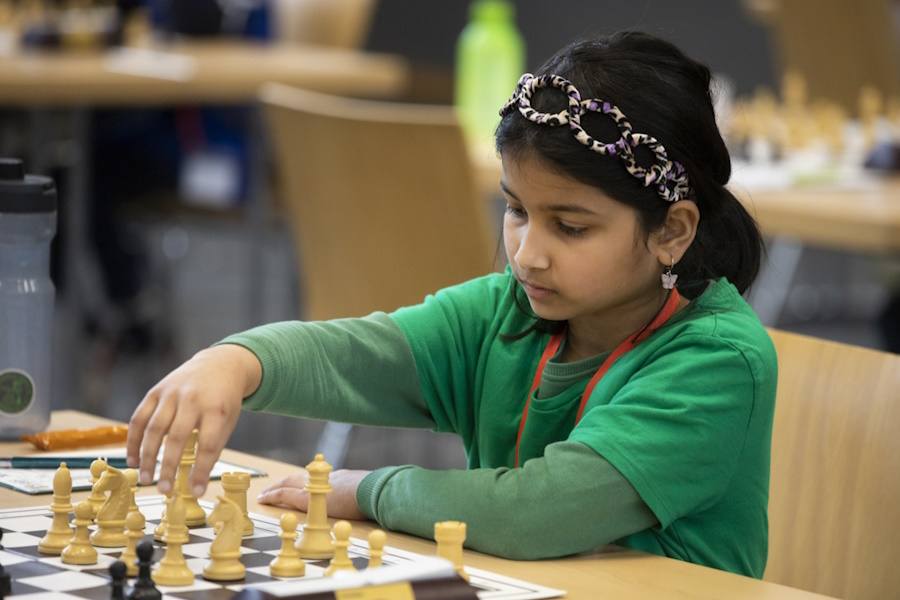
\includegraphics[width=\linewidth,height=0.5625\linewidth,keepaspectratio]{THJEM2.jpg}
    \captionof{figure}{Kashvi Bild}
    \label{fig:Kashvi Bild}
\end{center}

\subsection{Bild 2 - Hanna gegen Anna in Runde 1}
\begin{center}
    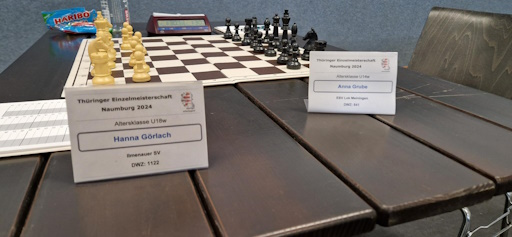
\includegraphics[width=0.8\linewidth,height=0.45\linewidth,keepaspectratio]{THJEM1.jpeg}
    \captionof{figure}{THJEM Hanna Schild}
    \label{fig:THJEM Hanna Schild}
\end{center}





\clearpage
\section{Partie von Kashvi}
Ich habe ein Teil der Partien digitalisiert. Leider lassen sich viele Partien aufgrund einer sehr schlechten Notation nicht eingeben. Der Jugendwart (Georg Lehmann) übernimmt dankenswerter WEise den Versuch die restlichen Partien zu digitalisieren.
\begin{itemize}
    \item[-] Lichess Studie: \url{https://lichess.org/study/XYIPdaoJ/xNqhky8Z}
\end{itemize}


\subsection{Partie ohne Anmerkungen}
Die PGN kann aus dem GitHub Repository heruntergeladen werden: \url{https://github.com/eskopp/IlmenauerSVBerichte/blob/main/2024_04_THJEM/unkommentiert.pgn}
\lstinputlisting{unkommentiert.pgn}
\clearpage

\subsection{Partie mit Anmerkungen}
Die PGN kann aus dem GitHub Repository oder Chessbase heruntergeladen werden: 
\begin{itemize}
    \item[-] \url{https://share.chessbase.com/SharedGames/share/?p=2i3CSGD4FhlwwzYYLm/2XVBB0h2sr1OZkzXpjB4f5HPCk09XDr3AjYnZKVjwOWgC}
    \item[-] \url{https://github.com/eskopp/IlmenauerSVBerichte/blob/main/2024_04_THJEM/kommentiert.pgn}
\end{itemize}

\lstinputlisting{unkommentiert.pgn}


\subsection{Schlussstellung}
\newchessgame
\fenboard{r1qkQ3/ppp4r/2Bp1p2/3N4/4P2p/P3p3/1PPN2PK/R7 b - - 2 22}
\chessboard
\end{document}
